% !TeX root = ../main-paper.tex
\section{Experimental Setup}


\begin{figure}[tb]
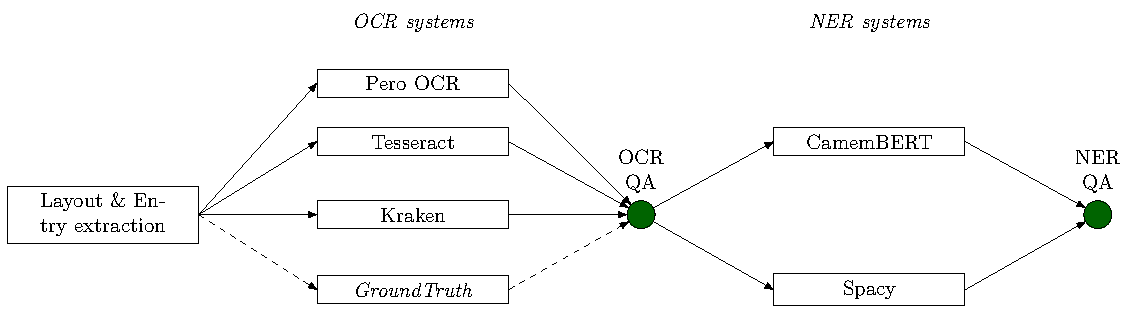
\includegraphics[width=\linewidth]{figs/protocol.pdf}
\caption{Scheme of the evaluation protocol.}
\label{fig.protocol}
\end{figure}

\subsection{Evaluation protocol \& Metrics}

\Cref{fig.protocol} depicts the evaluation procotol used to assess the OCR and NER systems. Two quality evaluation
are performed in the pipeline named respectively \emph{OCR Q.A.} and \emph{NER Q.A.}.

First the layout extraction and the entry segmentation of the page are performed with a semi-automated system and
checked by a human. Afterward, an OCR system runs on the thumbnails of each segmented entry to extract its text. An
entry might span over multiple text lines but is always single-block. Thus, the most adapted mode is chosen when
the OCR system allows for detection mode (e.g. the \emph{block} mode for \emph{Tesseract}). 

\textbf{OCR Q.A.} is performed after some text normalization of the OCR system outputs. Text normalization consists in
projecting unicode characters onto the latin-1 charset (whenever it makes sense) and removing extra symbols (hands,
crosses). Then, the predicted text is aligned with the reference text using standard tools and the Character Error Rates
(CER) are computed at entry level and at global level. 

\begin{align}
\mathrm{CER} &=  \frac{\#Errors}{\text{Reference Text Length}} & & \mathrm{CER}_\mathrm{norm} =  \frac{\#Errors}{\text{Alignment Length}} 
\end{align}

In this benchmark, we consider 3 OCR systems well-known for the historical document analysis: Pero OCR, Tesseract and Kraken. 

\edwin{FIXME: add ref papier eval OCR + ISRI, eval KRAKEN}


Next, a NER system extracts the named entities from the text of each entry output by the OCR and the \textbf{NER Q.A.}
is performed. The NER system outputs a text with tags that enclose the entities. To assess the quality of the entity
extraction, we rely on a technique similar as for the OCR evaluation. The predicted text is aligned with the reference
text and the tags are projected in the alignment. Then, the precision, recall and f-measure (or f-score) are computed considering
only the exact matches between entities. Precision and recall are defined by equation (2); the f-measure in their harmonic mean.

\begin{align}
    \mathrm{precision} &= \frac{\text{\#exact matches}}{\text{\#entries in prediction}} & \mathrm{recall} &= \frac{\text{\#exact matches}}{\text{\#entries in reference}}
\end{align}


The whole process is illustrated on~\cref{fig.eval-ocr-ner}. The OCR text and the GOLD text are first aligned to
evaluate the OCR accuracy. As there are 11 mismatches over 56 aligned characters, the CER is thus 24\%. This alignment
is then used to back-project the GOLD tags to build the tagged NER reference string. Finally, the NER system runs on the
OCR text; its output is compared to the NER reference string. There is only 2 over 3 tags matching in the prediction (precision),
while only 2 over 4 entities are matching in the reference (recall). It follows an overall f-score of 0.4.


\begin{figure}[tb]
    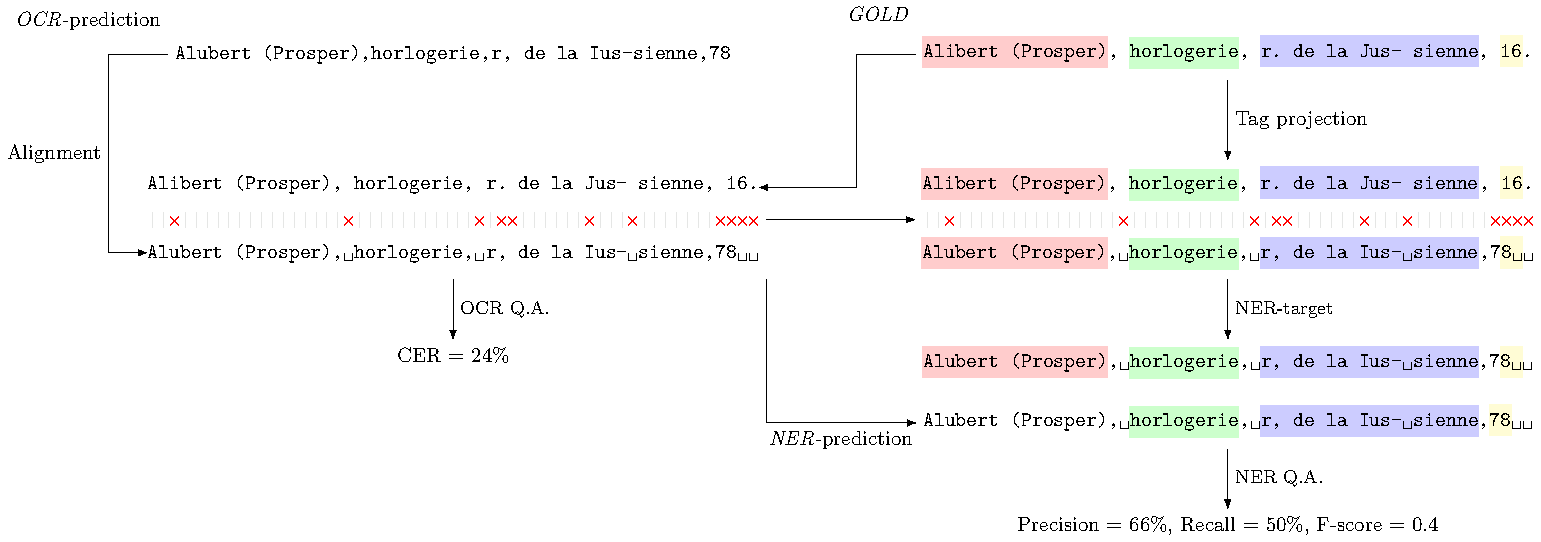
\includegraphics[width=\linewidth]{figs/eval-ocr-ner.pdf}
    \label{fig.eval-ocr-ner}
    \caption{OCR and NER evaluation protocol example.}
\end{figure}



\subsection{NER sensibility to the number of training samples}
\label{subsection:experiment-1}
The first experiment evaluates the performances of the three models on training sets of different sizes.
To do so, we split the gold reference into a training set, a development set, and a test set. The training set is then gradually reduced in size while maintaining the relative frequency of directories within.
The training and testing procedure is the same for the three models.

As the form and structure of entries varies across directory collections and through time, the model may learn to overfit on a subset of directories with specific features.
To reduce the evaluation bias, we start by leaving out 3 directories (1690 entries, ~20\%) from the gold reference to test each model on unseen directories.
Then a stratified sampling based on the entry directory name is applied to the remaining set to create a training (6373 entries, ~71\% of the gold reference) and a development set (709 entries, ~8\%).
This sampling procedure is a convenient way to shape both sets to reflect the diversity of directories within the gold reference.

To generate smaller training sets we start from the initial training set and iteratively split it in half using the same stratified sampling strategy as before.
We stop if there is only one entry left in a directory or if the current train set contains less than 30 entries.
Applying this procedure to the initial training set produced 8 training sets containing 49, 99, 199, 398, 796, 1593, 3186 and 6373 entries.

% Move to metrics ?
All metrics are evaluated on the test set, yet the biased model performances on the development sets are added in the article material for information.





\subsection{NER in noisy OCRed texts}
\label{subsection:experiment-2}
The second experiment assesses the impact of the OCR used on the quality of the NER results. To this end, we use directory entries whose text has been extracted, corrected and annotated manually (see Section 3). This reference text is aligned with the text produced on the same entries by Tesseract and PERO OCR. The named entities annotated in the reference text are then projected into the OCRed texts. To make sure that all training, development and test datasets contain the same annotations, only the entries for which the same number of annotations are found in the reference text and in the OCRised texts are kept. Finally, the reference text is divided into three datasets, using the same method as in Experiment 1. Two additional test files are generated with exactly the same entries as the test file produced from the reference text: one from the text produced by PERO OCR and one from that produced by Tesseract.




%\begin{itemize}
%\item At least 1 run per dataset, more if possible.
%\item Only use the best model; should be CamemBERT+pretrained
%\item Train on reference gold, evaluate on reference gold AND ocr-gold (2 datasets)
%\item split train/dev/test the same way than experiment 1. Use the exact same splitting %for datasets so the clean test set, pero test set and tesseract test sets contains the %same entries.
%\end{itemize}
 
 
%\begin{itemize}
%\item All : leave out 3 directories (~20\% of the dataset) as test data. Then apply stratified sampling based on the directory of each entry to split the remaining into a train set (~72\%) and a dev set (~8\%).
%\item Spacy CNN : No limit on epochs, instead use patience 1600.
%\item CamemBERT: 3 epochs.
%\item CamemBERT pretrained: 3 epochs, pretraining on MLM + NSP with ~20000 raw texts extracted with Pero-OCR.
%\end{itemize}




\subsection{Implementation details}

\subsubsection{OCR systems parameters}
\nathalie{Y a-t-il des précisions à ajouter sur la façon dont ont été utilisés les OCR? Ou bien ce sont les versions "sur étagère" qui ont servi?}
\joseph{Totalement sur l'étagère. On a normalisé un peu les données après, c'est tout.}
\begin{itemize}
    \item Tesseract 4.1.1 (newest version: 5, released Nov. 2021)
    \item Pero OCR version from git repo, master branch updated on Sep 15, 2021 % 8b20f29    
    \item other?  % kraken if times allows
\end{itemize}

Pero OCR uses ParseNet \joseph{TODO ref} as internal layout parser for line detection.
Pero OCR uses an LSTM engine \joseph{TODO check + ref} for text line recognition.
Pero OCR generally works very well, as long as the bounding boxes of the regions to recognize are not too tightly adjusted.
Trained on newspapers in European languages by its development team.
Can output results in Latin, Greek and Cyrillic scripts, as well as some commonly-used typographic symbols.

% PERO refs
% O Kodym, M Hradiš: Page Layout Analysis System for Unconstrained Historic Documents. ICDAR, 2021.
% M Kišš, K Beneš, M Hradiš: AT-ST: Self-Training Adaptation Strategy for OCR in Domains with Limited Transcriptions. ICDAR, 2021.
% J Kohút, M Hradiš: TS-Net: OCR Trained to Switch Between Text Transcription Styles. ICDAR, 2021.


\subsubsection{Spacy}
We use the French model \textit{fr\_core\_news\_lg} provided by Spacy\mcite{spacy} library and leverage the library utilities to fine-tune it with various training and validation datasets derived from our ground truth dataset (see section 5.2 for details). The base model is fine-tuned in turn with each of the 8 generated training datasets, using the same training parameters. Early stopping is activated with patience parameters set at 1600. For each size of training dataset, 5 runs are performed, always with the same parameters, and the mean value of each performance score is computed.

%and Huggingface for the BERT 
%tok2vec(words embeddings + encoding) + attention layer  +  transition-based %model.

\subsubsection{Huggingface CamemBERT}
We start from the CamemBERT-ner model already fine-tuned on WikiNER-fr corpus and published on the Hugging Face repository \footnote{\url{https://huggingface.co/Jean-Baptiste/camembert-ner}}. Its output layer is a linear model with a Softmax function. Four NER models are derived from this base model: 

\textit{BERTreference} The base model is fine-tuned in turn on each of the training datasets generated from the groundtruth corpus. Training parameters are set depending on the considered experiment: early stopping is activated with patience parameter set at 3 for experiment 1 and at 5 for experiment 2. \nathalie{<-- bertrand tu peux vérifier si c'est OK stp?}

\textit{BERTpero-ocr} This model is used for experiement 2 only. The base model is fine-tuned on the training dataset generated by projecting the named entities annotation on the text extracted by PERO OCR, using the same parameters as for the \textit{BERTreference} model.

\textit{BERTptrn-reference} The base model is pretrained on 845 000 entries extracted with PERO OCR for the Next  Sentence  Prediction  (NSP) and  Masked  Language  Model(MLM) tasks. Then it is fine-tuned with the parameters and on the same training datasets as the \textit{BERTreference} model.

\textit{BERTptrn-pero-ocr} The base model is pretrained like the \textit{BERTptrn-reference} model. Then it is fine-tuned with the parameters and on the same training datasets as the \textit{BERTpero-ocr} model.

The source code of all our experiments is publicly available on the following repository \url{lien github}.